\subsubsection{Hybrid Emulator}

\YIComment{Do this}

\YIComment{Do mips comparison with JIT}

\YIComment{Do execution time comparison with JIT}

\YIComment{Write about different hybrid variants and performance characteristics of -L and -LS}

\YIComment{Write about different -T values}

\begin{figure}[H]
    \centering
    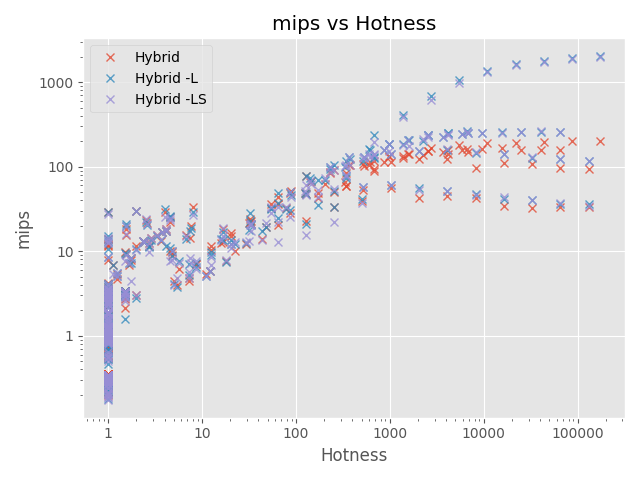
\includegraphics[scale=0.75]{output/graphs/scatter/hybrid/hotness.png}
    \caption{Performance (mips) vs hotness for all tests on the hybrid emulators.}
    \label{figure:hybrid-hotness}
\end{figure}

\autoref{figure:hybrid-hotness} shows how the performance of the hybrid emulator changes with relationship to the hotness of the programs; unlike the JIT, which has a monotonic relationship, the hybrid shows a more complex relationship.

This is because hybrid behaves like an interpreter for sufficiently cold tests, but like a JIT for sufficiently hot tests. This causes it to exhibit the `flat' performance profile of the interpreter for low hotness, before dropping in performance then rising as the JIT would. The dip in performance or the inflection point is where the hybrid begins to act like a JIT, and thus takes on all the associated overheads of a JIT, without having time make them worthwhile. This region therefore performs worse than both the interpreter or the JIT.

Naturally, we should expect the location of this inflection point to change with \texttt{-T}. Since \texttt{-T} determines how many times a block must be executed before it is compiled, it roughly corresponds to how hot a block should be before the hybrid begins emulating like a JIT; given this, we would expect the inflection to occur at higher hotness values for higher \texttt{-T}.

\YIComment{Show how that relationship changes with -T}

The ideal configuration found for the Hybrid emulator is detailed in \autoref{tbl:hybrid-optimal}

\begin{table}[H] 
    \centering
    \begin{tabular}{l|c}
        \toprule
        Option & Value \\
        \midrule
        \texttt{-L} & \cmark \\
        \texttt{-S} & \xmark \\
        \texttt{-T} & 10 \\
        \bottomrule
    \end{tabular}
    \caption{Optimal configuration found for the Hybrid emulator.}
    \label{tbl:hybrid-optimal}
\end{table}